\begin{savequote}[75mm]
Searle may only be behaving \textit{as if} he were thinking deeply about these matters. But, even though I disagree with him, his simulation is pretty good, so I'm willing to credit him with real thought.\qauthor{Nils Nilsson}
\end{savequote}

\chapter{Luna Rating Prediction}

\section{Introduction}
\subsection{The Luna Rating Prediction Problem}
In the previous chapter, I discussed the machine learning problems implicit in the Interview and Response Phases of the Luna Game. This chapter addresses the remaining problem implied by the Guess Phase. Consider the typical behavior of a human player during this phase. The player observes her opponent's responses. If she has asked the same questions to previous opponents, she may compare these new responses to old responses, and conjecture that opponents who respond similarly have similar Smarts Ratings. In addition, she may compare these new responses directly with the ideal responses that she had in mind, reasoning that opponents who provide nearly ideal responses are likely to have high Smarts Ratings. After taking into account all the information at her disposal --- previously observed responses and previously conceived ideal answers --- she hazards a guess.

The task implicit in the Guess Phase is best clarified in terms independent from the Luna Game. The goal is to learn a mapping from ordered sets of natural language responses to a bounded subset of the real numbers that minimizes ($L_1$) error on test data. Without loss of generality, one can assume that the target space is $[0, 1] \subset \mathbb{R}$. Let $q$ be the number of natural language responses per input, i.e. the number of questions. Let $\mathcal{F}$ be a set of features. For a given input, and a given response in that input, let $f_1, ..., f_k$ be the active features. This response can be represented sparsely as the sum of one-hot vectors: $\mathbf{x_j} =\sum_{i=1}^k \delta(f_i)$, where $\delta$ gives the one-hot encoding of an index with dimension $d_{in} = |\mathcal{F}|$. The full input can then be represented as a vector $\mathbf{x}$ of dimension $q\cdot d_{in}$, with each of the sparsely represented responses concatenated together. Training data are given as $\{\mathbf{x}_i, y_i\}$, where the $\mathbf{x}_i$ are vectors of the described form, and $y_i \in [0, 1]$. This representation is illustrated in Figure \ref{fig:lrpformalization}. Features may also be real-valued, rather than binary. In this case, features contain both an index and a separately value, and the one-hot encoding of an active feature is multiplied by its corresponding value.

\begin{figure}[h]
\centerline{%
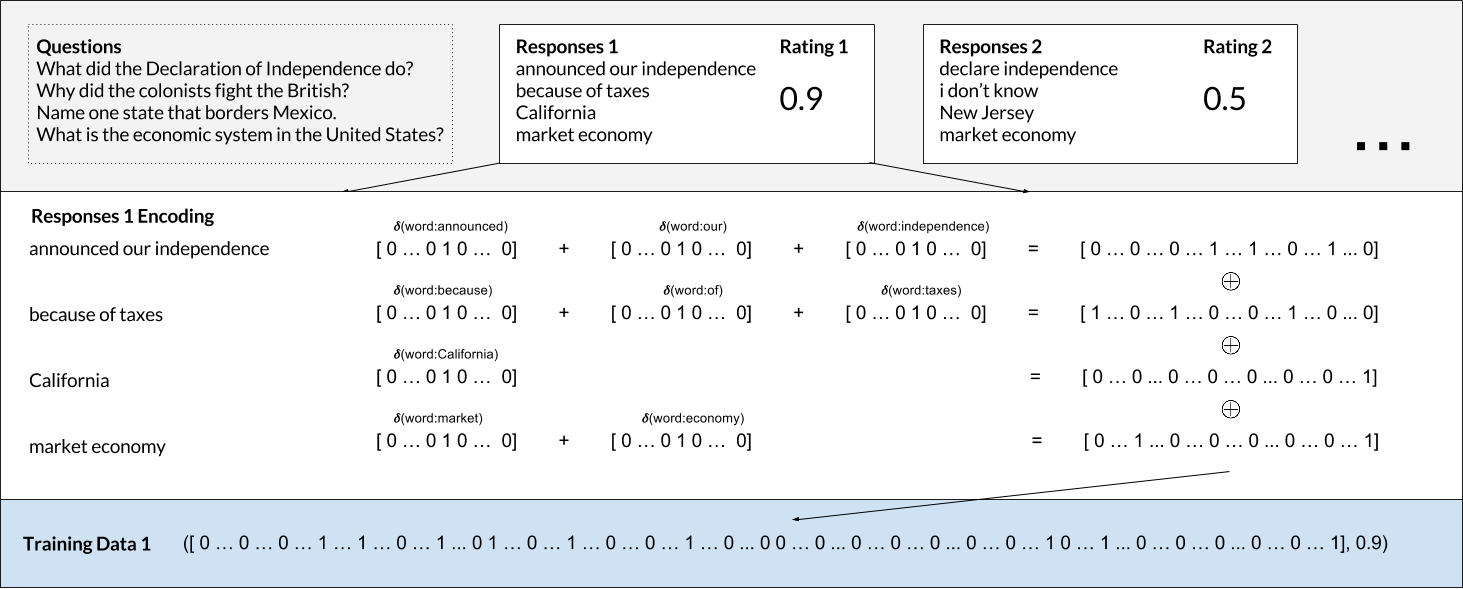
\includegraphics[width=0.95\textwidth]{figures/lrpformalization.png}%
}%
\caption{Training data representation in Luna Rating Prediction. Each input is an ordered set of natural language responses to a fixed set of questions. Each response is encoded by the sum of one-hot vectors of the features active in the response. In this example, features are simply unigrams. The encoded responses are concatenated together to form the final input representation. The training data consists of this input representation and the corresponding target rating, which is a real value between $0$ and $1$ inclusive.}
\label{fig:lrpformalization}
\end{figure}

Note that the formalization of the problem thus far makes no mention of an answer key. One might be tempted to incorporate an answer key by converting it into an instance of training data with a target rating of $1.0$. However, this conversion would lead to a critical loss of information. The rating for a set of responses is assigned with possible reference to the answer key, which is determined \textit{a priori}. In other words, while training data are assumed to be derived independently from an identical distribution, the answer key is actually not independent from other rated responses. Therefore the characterization of the problem should treat the answer key separately from other training data. Formally, I will say that the problem is \textit{parameterized by an answer key}, which is an ordered set of natural language responses encoded in the same manner as other responses. This completes the formalization.

Given the inspiration of this problem, I call it the Luna Rating Prediction (LRP) problem. LRP avoids some of the difficulties of natural language understanding, but also introduces a host of new challenges. For example, it is possible in principle to achieve very good results on LRP without a complete understanding of the natural language responses being analyzed. On the other hand, a complete understanding of the responses is not sufficient to solve LRP, since ratings must still be predicted. Machines may excel at mapping representations of responses to ratings, while humans may excel at representing the responses. A method for LRP must excel at both tasks. In this chapter, I present a collection of simple experiments to establish a baseline for the problem. I conclude with a discussion of avenues for future work and an argument for LRP's general applicability beyond the scope of Luna.

\subsection{Related Work}
LRP may be viewed as a relaxed version of a problem that has been previously considered: Automatic Short Answer Grading (ASAG)  \citep{burrows2015eras, pulman2005automatic, sukkarieh2009c, ziai2012short}. Motivated by standardized testing, ASAG attempts to automatically grade students' natural language responses to a fixed set of questions. While LRP is concerned only with a single target rating for a particular input, ASAG requires scores for each question. In other words, the target space of ASAG is $[0, 1]^q$, whereas the target space of LRP is $[0, 1]$. The two problems are otherwise identical. A method for ASAG may be applied to LRP using a mapping from $[0, 1]^q$ to $[0, 1]$; such a mapping could be learned from data, or it could simply be a normalized summation. However, if one is starting from scratch, it is simpler to approach LRP directly without considering ASAG as an intermediate problem. For example, suppose that one question is much more predictive of target ratings than other questions. A method for LRP would be able to leverage this correspondence, while ASAG would still require accurate ratings for each of the individual questions irrespective of informativeness.

While the two problems deserve separate treatments, previous work on ASAG can still inform future work on LRP. A recent review by Burrows et al. summarizes advances in ASAG, drawing upon over $80$ papers with $35$ distinct systems  \citep{burrows2015eras}. These systems differ in their natural language processing techniques, model building, grading models, and effectiveness. Each of these systems could be potentially adapted for LRP, offering several possible avenues for future research. Here I focus on the state-of-the-art system developed by Education Testing Services \citep{heilman2013ets}. This system serves both as a representative example of ASAG systems and as a starting point for LRP. The system performs Logistic Regression to classify responses as correct or incorrect based on two categories of features: word and character n-gram features, and text similarity features between response and answer key or response and other responses. It also groups questions into different problem domains and then uses a ``domain adaptation'' technique, which introduces three separate copies of each feature for generic, domain-specific, and question-specific weighting. This straightforward Logistic Regression approach outperforms all other existing techniques on the two tested datasets. The general approach of defining a wide variety of natural language features and training a linear model is common among competing systems.

\section{Methods}
\subsection{Datasets}
I use two datasets to evaluate various approaches to LRP. Both datasets are comprised of responses to standardized tests with short answer questions. The first dataset was introduced by \citet{basu2013powergrading} in their work on computer-assisted grading. They created the dataset by posing $20$ questions from the $2012$ United States Citizenship Exam to workers on Amazon Mechanical Turk, collecting a total of $698$ responses. $10$ of the questions were selected for grading by three human judges, who marked each answer as each correct or incorrect. I refer to this dataset as the ``Powergrading'' dataset, derived from the name of the system that  \citet{basu2013powergrading} developed.

The second dataset I use for LRP was introduced by \citet{mohler2011learning} in their work on ASAG. These data consist of responses to short answer problem set and exam questions in a Data Structures course at the University of North Texas. In total, the dataset contains $24$ complete responses to $87$ questions. Responses are graded by two human judges on a scale from $0$ to $5$, and these two grades are averaged together per question. I refer to this dataset as the ``Mohler $11$'' dataset. Responses in this dataset are typically longer and more involved than responses in the Powergrading dataset. This level of natural language, combined with the relatively small number of samples, makes the Mohler dataset significantly more challenging for LRP than the Powergrading dataset.

Since they were collected for ASAG, neither of these datasets are immediately in the format required for LRP. In particular, each question is graded individually, as opposed to each respondent possessing an overall rating. To convert to LRP, I simply add all grades for each respondent and discard the per-question grades. Next I normalize these overall respondent ratings so that all ratings are on a scale of $0$ to $1$. The final rating preprocessing step is splitting into training and test sets at a ratio of $4$ to $1$ respectively. To preprocess text responses, I remove all punctuation, stop words, and convert all remaining characters to lowercase.

\begin{figure}[h]
\centerline{%
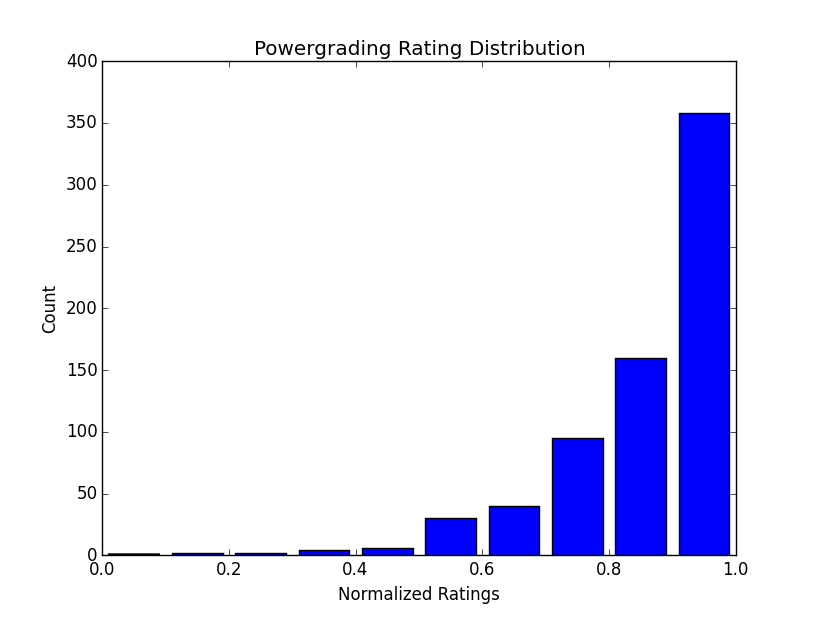
\includegraphics[width=0.5\textwidth]{figures/powerGradingDistribution.png}%
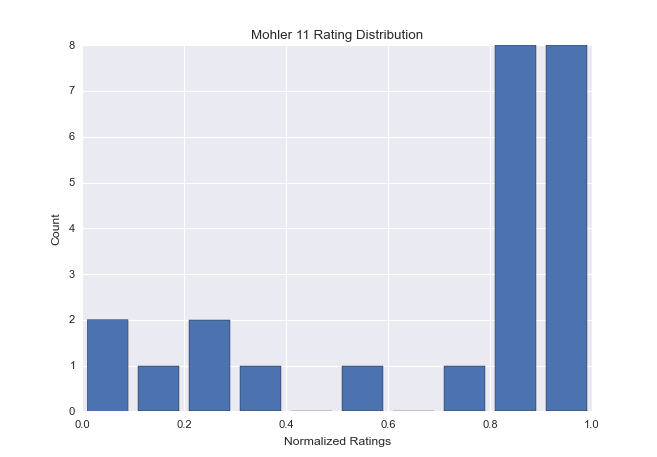
\includegraphics[width=0.5\textwidth] {figures/mohlerRatings.png}%
}%
\caption{Normalized ratings for the two datasets used for evaluating approaches to the Luna Prediction Rating problem. The Powergrading dataset, comprised of responses to a subset of the $2012$ United States Citizenship Exam, was introduced by \citet{basu2013powergrading}. The Mohler $11$ data, comprised of responses to problem set and exam questions in a University of North Texas Data Structures course, was introduced by \citet{mohler2011learning}. Ratings were computed by summing individual question grades and normalizing.}
\label{fig:RatingDistribution}
\end{figure}

\subsection{Features}

Beyond stating LRP as a new problem for the machine learning community, the main contribution of this chapter is a thorough exploration of approaches to the problem. Following the recent work done on ASAG, my strategy is to associate several features with each set of responses, which can be subsequently used for regression. I divide the feature definitions into two categories: question-based features and response-based features. The former takes into account answer keys, while the latter focuses on data provided by previous rated respondents. I then experiment with several types of regression to combine the features for an optimal model.

\subsubsection{Question-Based Features}
Question-based features exploit the relationship between the answer key and the training data. A statistical approach would model the conditional probability distribution of ratings given responses and ideal responses. Such an approach would not initially presume any relationship between responses and ideal responses; rather, this relationship would be learned from training data. Here I take advantage of the intuitive relationship between responses and ideal responses, leaving the statistical approach as an avenue for future work. For the purpose of predicting target ratings, the most important aspect of the relationship between responses and ideal responses is \textit{semantic similarity}. If a set of responses is close in meaning to the ideal responses of the answer key, one would expect a high target rating. The question-based features I consider in this chapter are defined according to various measures of semantic similarity between given and ideal responses. 

Measuring semantic similarity between two samples of natural language is a difficult task. If the two sentences differ only in word order, or only in a few words, then simple approaches can reliably detect similarity. By considering synonyms of the words in both sentences, the similarity measure may be improved. However, in many cases, it is impossible to accurately capture similarity without a deeper semantic understanding of the two sentences. One common approach for representing semantic similarities is to infer vector representations for words, referred to as word embeddings,and then to calculate similarity based on some geometric measure, such as cosine similarity. I include features based on these word embeddings in addition to simpler unigram-based features. 

The full list of considered question-based features is below. Each feature is a function of a response and is implicitly parameterized by the corresponding ideal response.

\begin{enumerate}
\item \textbf{Binary Word Overlap (BWO)}: This feature gives $1$ if the response contains at least one of the words in the ideal response and $0$ otherwise.
\item \textbf{Fraction Word Overlap (FWO)}: This feature gives the number of words that appear in both the response and the ideal response, divided by the cardinality of the union of both sets.
\item \textbf{Character Edit Distance (CED)}: This feature is based on the edit distance (Levenshtein distance) between the response and the ideal response at the level of characters. The feature gives $1.0$ minus the fraction of the edit distance and the length of the larger string.
\item \textbf{Word Edit Distance (WED)}:  This feature is based on the edit distance (Levenshtein distance) between the response and the ideal response at the level of words. For example, the word edit distance between ``hello, world'' and ``goodbye, moon'' is $2$. The feature gives $1.0$ minus the fraction of the edit distance and the greater number of words in either string.
\item \textbf{Word2Vec Cosine Similarity (WCS)}: I use pre-trained word embeddings from the Penn Treebank corpus and simply average all of the word embeddings for the given response and ideal response. Then this feature gives the cosine similarity between these two vectors.
\item \textbf{Semantic Nets (Li et al.) (SNL)}: For a more sophisticated approach to short sentence similarity, I refer to the work of \citet{li2006sentence}. They offer a comprehensive metric that takes into account lexical, semantic, and syntactical information about the two sentences being compared\footnote{One immediate downside of this feature is that it takes significantly more time to compute than any other feature described in this chapter. The results pertaining to this feature alone took nearly 10 days to generate on a single CPU.} I use an existing Python implementation of SNL that uses the English corpora provided by \citet{bird2009natural}. The output of their similarity measure is a value between $0$ and $1$. Thus this feature gives the calculated similarity between the response and ideal response.
\end{enumerate}

For future work on developing question-based features for LRP, it may be worthwhile to adapt methods for two related problems: paraphrase detection and textual entailment. Paraphrase detection assesses whether one sample is a paraphrase of the other. Textual entailment is the task of detecting whether one sample of natural language logically implies another sample. For the purpose of LRP, one might like to give high ratings to players whose responses imply the answer key, even if they are not exactly the same. Both of these problems are active areas of research in natural language processing and new results will likely be relevant to LRP as well.

\subsubsection{Response-Based Features}
Response-based features capture the direct relationship between responses and target ratings without reference to the answer key. Any traditional feature of a natural language sentence may be used as a response-based feature. The goal is to concisely and quantiatively represent aspects of responses that influence target ratings. For example, if the value of a response is entirely based on whether or not it contains a particular word, then an appropriate response-based feature would assign a $1$ to responses containing that word and a $0$ otherwise. I include this simple bag-of-words feature and several others in my predictive model. The full list of response-based features follows.

\begin{enumerate}

\item \textbf{Bag of Words (BOW)}: There is one BOW feature per word in the vocabulary induced by the dataset. Each BOW feature is active when its word is present anywhere in the given response.

\item \textbf{Bigrams (BIG)}: There is one BIG feature per bigram (two consecutive words) for all bigrams in the dataset. Each BIG feature is active when its bigram is present anywhere in the given response.

\item \textbf{Bag of Synsets (SYN)}: There is one SYN feature per word in the vocabulary induced by the dataset. 
Each SYN feature is active when any of the synonyms of its word are present anywhere in the given response. Synonyms are determined via WordNet \citep{fellbaum1998wordnet}. 

\item \textbf{Nearest Neighbor via Overlap (NNO)}: This feature is set according to the target rating of the training response that is most similar to the given response, where similarity is defined as the number of overlapping words.

\item \textbf{Nearest Neighbor via Character Edit Distance (NNC)}: This feature is the same as NNO, except similarity is defined by character edit distance rather than overlap.

\item \textbf{Nearest Neighbor via Word Edit Distance (NNW)}: This feature is the same as NNO, except similarity is defined by word edit distance rather than overlap.


\end{enumerate}

\subsection{Regression}
With features defined, the task then takes the standard form of a regression problem. For simplicity, I assume here that the rating is a linear combination of the features. I then consider two models of regression. The first is Ordinary Least Squares Linear Regression, which minimizes the sum of squares between predicted and actual ratings. I then run Lasso Regression $(\alpha = 0.1)$, which biases towards simpler models by penalizing the number of nonnegative coefficients in favor of sparse solutions. In both cases, I use the implementations in the Scikit-Learn library for machine learning  \citep{pedregosa2011scikit}.
\section{Results}
I ran OLS Linear Regressions and Lasso Regressions on each of the $12$ features for $100$ trials. In addition, I included a combination of all $12$ features (COM), and two controls. The first control predicts a random rating for a given set of responses (RAN). The second control, which I refer to as the ``constant best guess'', always predicts the average of all previously seen ratings (CBG). To consider a feature useful, it should at least outperform both of these controls on average. I define performance in terms of the Root Mean Square Error between predicted ratings and actual ratings in the test set. The results of these experiments are depicted in Figure 2. Lasso Regression yielded no meaningful differences from OLS, so I depict only the latter.
\begin{figure}[h]
\centerline{%
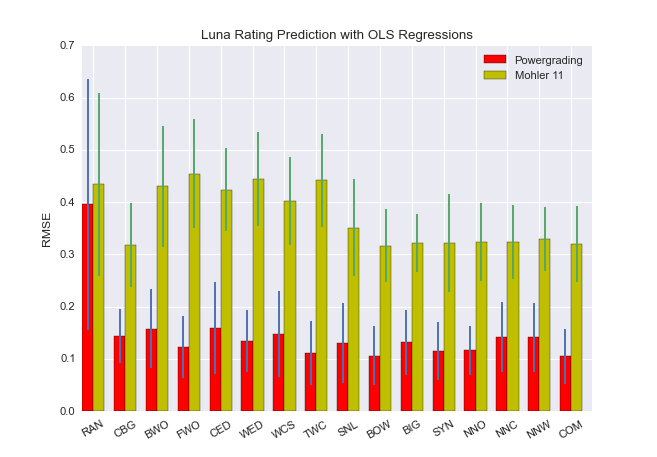
\includegraphics[width=0.9\textwidth]{figures/ratingPredictionFinalResults2.png}%
}%
\caption{Fifteen approaches to the Luna Prediction Rating problem on two datasets using Ordinary Least Squares Linear Regression. From the left, the first two approaches represent baseline controls; the following six approaches are each OLS Linear Regressions on single question-based features; the following six are also OLS Linear Regressions, but on single response-based features instead; the last is an OLS Linear Regression that includes all $12$ previous features. The Root Mean Square Error averaged over $100$ trials is plotted for each approach. Refer to the text for the feature abbreviations.}
\label{fig:RatingDistribution}
\end{figure}

The relative performances of the approaches seem to be consistent between the two datasets tested. As expected, the Mohler $11$ dataset proves far more difficult, likely due to the very limited size of the training set, the large number of responses per respondent, and the longer length of each response. Also unsurprising is the result that for OLS Linear Regression, a combination of all features outperforms any single feature. The combination does not perform as comparably well in Lasso Regression, presumably because the number of features actually included is small due to the penalty term. In both cases, any margin of improvement offered by a combination of all features is slim. Simple response-based features such as Bag of Words or Nearest Neighbor via Overlap are competitive with the combination. In practice, it may be preferable to use one or both of these due to the savings in computational resources. Among the question-based features, Binary Word Overlap fares the best, but cannot outperform the Constant Best Guess baseline. In future work, the question-based features could likely be improved by augmenting the answer keys with semantically equivalent answers.

\section{Discussion}
In this chapter, I defined the Luna Rating Prediction problem of predicting target values from ordered sets of natural languages responses and an answer key. I discussed the closely related problem of Automatic Short Answer Grading and demonstrated how datasets and methods for ASAG can be adapted for LRP. I then presented initial work on LRP, which centered around several features of response sets that I use to learn a model for predicting ratings. These features were presented in two categories: question-based features, which rely only on a preset answer key, and response-based features, which ignore the answer key but take advantage of seen responses from previous rated respondents. I combined these features using traditional regression techniques to arrive at a comprehensive system for LRP.

For a player of the Luna Game, the ability to solve LRP is critical. The outcome of a Game hinges on the difference between predicted ratings and actual ratings. A human player may take advantage of the machine learning approaches to LRP offered here, but more likely the human will learn to rate well after several rounds of play without any formalisms or explicit machine learning techniques. This human ability is based on an understanding of natural language, a deep knowledge base, and the relative ease with which humans judge one another in everyday scenarios. As machine players build an understanding of natural language and a knowledge base from answering questions in the Luna Game, these advances should be transferrable to LRP as well. A truly intelligent player of the Luna Game is unlikely to consider LRP and question answering as completely separate problems, but rather as manifestations of one general underlying problem.

Throughout this chapter, I sought to treat LRP as a general problem beyond the scope of the Luna Game, since I expect work on the problem to have several applications. Any situation in which a judge wishes to automatically evaluate a respondent can be thought of as an instance of LRP. The quantity being evaluated may be completely known to the respondent, as is the case in the Luna Game. However, in some applications, the quantity may be only partially known or unknown. For example, consider the case of a government official wishing to estimate the probability that a convict will repeat an offense based on questionnaire responses, or the case of an health insurance company wishing the estimate the amount of money that a customer will require for medical care. These real life applications combined with the motivation provided by the Luna Game make LRP a problem worthy of further study.
